



Une grande différence quand on utilise un modèle de RLM au lieu de la RLS, c'est qu'on peut créer des modèles plus complexes. On verra ici deux façons pour ce faire, soit inclure des variables catégoriques et inclure des interactions.

\section{Variables exogènes catégoriques}

Jusqu'à maintenant, nous n'avons considéré que des variables
exogènes continues. Il arrive pourtant souvent en pratique que
les variables exogènes ne puissent prendre des valeurs que dans
un ensemble de valeurs possibles, et que ces valeurs n'impliquent
pas un ordre entre les mesures. Quelques exemples:
\begin{eqnarray*}
x_{1i}&=&\left\{\begin{array}{ll} H, & \mbox{si $i$ est un homme}\\
F, & \mbox{si $i$ est une femme}\end{array}\right.\\
x_{1i}&=&\left\{\begin{array}{ll} 1, & \mbox{si $i$ est une ville}\\
-1, & \mbox{si $i$ est un village}\end{array}\right.\\
x_{1i}&=&\left\{\begin{array}{ll}1, & \mbox{si $i$ est à ON}\\
0, & \mbox{si $i$ est à OFF}\end{array}\right.\\
\end{eqnarray*}

On peut simplement ajouter une variable catégorique linéairement dans le modèle de RLM. La valeur de cette variable modifiera l'ordonnée à l'origine de la régression. Il faut toutefois faire attention à la façon avec laquelle on code les variables catégoriques pour s'assurer que le modèle soit facile à interpréter.

\newpage
\textbf{Variable dichotomique}

Dans le cas d'une variable dichotomique, il est toujours plus prudent de coder $x_i$ sous la forme d'une variable indicatrice, c'est-à-dire sous la forme
$$x_i=\left\{\begin{array}{ll} 1, & \mbox{si ...}\\
0, & \mbox{sinon}\end{array}\right.$$

Si ce type de codage n'est pas utilisé, alors les $\beta$ peuvent \^etre difficiles à
interpréter.

Par exemple si
$$x_{i}=\left\{\begin{array}{ll}-5, & \mbox{si $i$ est un homme}\\
5, & \mbox{si $i$ est une femme}\end{array}\right.$$
Alors le modèle $Y_i=\beta_0+\beta_1 x_i+\varepsilon_i$ nous donne
\begin{eqnarray*}
\esp[Y_i|\mbox{$i$ est un homme}]&=&\beta_0-5\beta_1\\
\esp[Y_i|\mbox{$i$ est une femme}]&=&\beta_0+5\beta_1
\end{eqnarray*}
On a donc que $\beta_0$ est la moyenne des espérances de $Y$ pour les hommes et les femmes, et $\beta_1$ représente 0.1 fois la différence entre la valeur moyenne de $Y$ pour les hommes et celle pour les femmes.

Si on prend plutôt
$$x_{i}=\left\{\begin{array}{ll}1, & \mbox{si $i$ est un homme}\\
0, & \mbox{si $i$ est une femme}\end{array}\right.$$ alors on a
\begin{eqnarray*}
\esp[Y_i|\mbox{$i$ est un homme}]&=&\beta_0+\beta_1\\
\esp[Y_i|\mbox{$i$ est une femme}]&=&\beta_0
\end{eqnarray*}
et maintenant $\beta_0$ est simplement la valeur moyenne de $Y$ pour les femmes et  $\beta_1$ représente exactement la différence entre la valeur moyenne de $Y$ pour les hommes et celle pour les femmes.

Un autre codage souvent utilisé durant la collecte de données est de la forme

$$x_{i}=\left\{\begin{array}{ll}1, & \mbox{si $i$ est un homme}\\
2, & \mbox{si $i$ est une femme}\end{array}\right.$$

Dans ce cas, $\beta_1$ s'interprète de la même façon qu'avec la variable indicatrice, mais $\beta_0$ est plus complexe à interpréter.

\textbf{Variable polytomique}

Si $x$ est une variable polytomique, c'est-à-dire que $x_i$ peut
prendre une parmi $C\ge2$ valeurs possibles, la fa\c{c}on prudente
de procéder est de définir $C-1$ variables indicatrices.
Ainsi,
si $$x_{1i}=\left\{\begin{array}{ll} 1, & \mbox{si $i$ est bleu}\\
2, & \mbox{si $i$ est rouge}\\ 3, & \mbox{si $i$ est jaune}\\ 4, &
\mbox{si $i$ est vert}\end{array}\right.$$ alors on définit
\begin{eqnarray*}
x_{Bi}&=&\left\{\begin{array}{ll}1, & \mbox{si $i$ est bleu}\\ 0,
& \mbox{sinon}\end{array}\right.\ \ \
x_{Ri}=\left\{\begin{array}{ll}1, & \mbox{si
$i$ est rouge}\\ 0, & \mbox{sinon}\end{array}\right.\\
x_{Ji}&=&\left\{\begin{array}{ll}1, & \mbox{si $i$ est jaune}\\
0, & \mbox{sinon}\end{array}\right.\end{eqnarray*} Dans ce cas
\begin{eqnarray*}
x_{1i}=\mbox{bleu}&\Rightarrow&(x_{Bi},x_{Ri},x_{Ji})=(1,0,0)\\
x_{1i}=\mbox{rouge}&\Rightarrow&(x_{Bi},x_{Ri},x_{Ji})=(0,1,0)\\
x_{1i}=\mbox{jaune}&\Rightarrow&(x_{Bi},x_{Ri},x_{Ji})=(0,0,1)\\
x_{1i}=\mbox{vert}&\Rightarrow&(x_{Bi},x_{Ri},x_{Ji})=(0,0,0)
\end{eqnarray*}
Ainsi, si
$Y_i=\beta_0+\beta_{B}x_{Bi}+\beta_Rx_{Ri}+\beta_Jx_{Ji}+\varepsilon_i$,
\begin{eqnarray*}
\esp[Y_i|\mbox{$i$ est bleu}]&=&\beta_0+\beta_B\\
\esp[Y_i|\mbox{$i$ est rouge}]&=&\beta_0+\beta_R\\
\esp[Y_i|\mbox{$i$ est jaune}]&=&\beta_0+\beta_J\\
\esp[Y_i|\mbox{$i$ est vert}]&=&\beta_0.
\end{eqnarray*}


\begin{remarque}
Si une variable exogène ne prend que très peu de valeurs différentes, il est important de déterminer s'il s'agit d'une variable continue pour laquelle on a peu de mesures ou s'il
s'agit d'une variable polytomique. Selon la façon avec laquelle la variable est incluse dans le modèle, l'interprétation sera différente, ainsi que l'information qu'on pourra retirer du modèle.
\end{remarque}

\newpage
\begin{exemple}
\label{eg:lot}
Soit $x_{1i}$, le numéro de lot du produit $i$, $x_{2i}$, la
concentration de sel dans le produit $i$ et $Y_i$, l'indice de
qualité du produit $i$. Les variables $Y_i$ et $x_{2i}$ sont des
variables continues, alors que $x_{1i}$ est un variable
polytomique prenant une des valeurs $\{1,2,3,4\}$.

On ajuste le modèle
$$Y_i=\beta_0+\beta_{11}x_{11i}+\beta_{12}x_{12i}+\beta_{13}x_{13i}+\beta_2x_{2i}
+\varepsilon_i,$$ o\`u
\begin{eqnarray*}
x_{11i}&=&\left\{\begin{array}{ll} 1, & x_{1i}=1\\
0, & x_{1i}\neq1\end{array}\right. \ \ \
x_{12i}=\left\{\begin{array}{ll} 1, & x_{1i}=2\\
0, & x_{1i}\neq2\end{array}\right. \\
x_{13i}&=&\left\{\begin{array}{ll} 1, & x_{1i}=3\\
0, & x_{1i}\neq3.\end{array}\right.\end{eqnarray*}

La figure \ref{figex81} illustre graphiquement ce modèle. Notez qu'on suppose dans la figure que tous les coefficients sont positifs, mais ce n'est absolument pas nécessaire en pratique.

\begin{figure}[H]
\begin{center}
\centerline{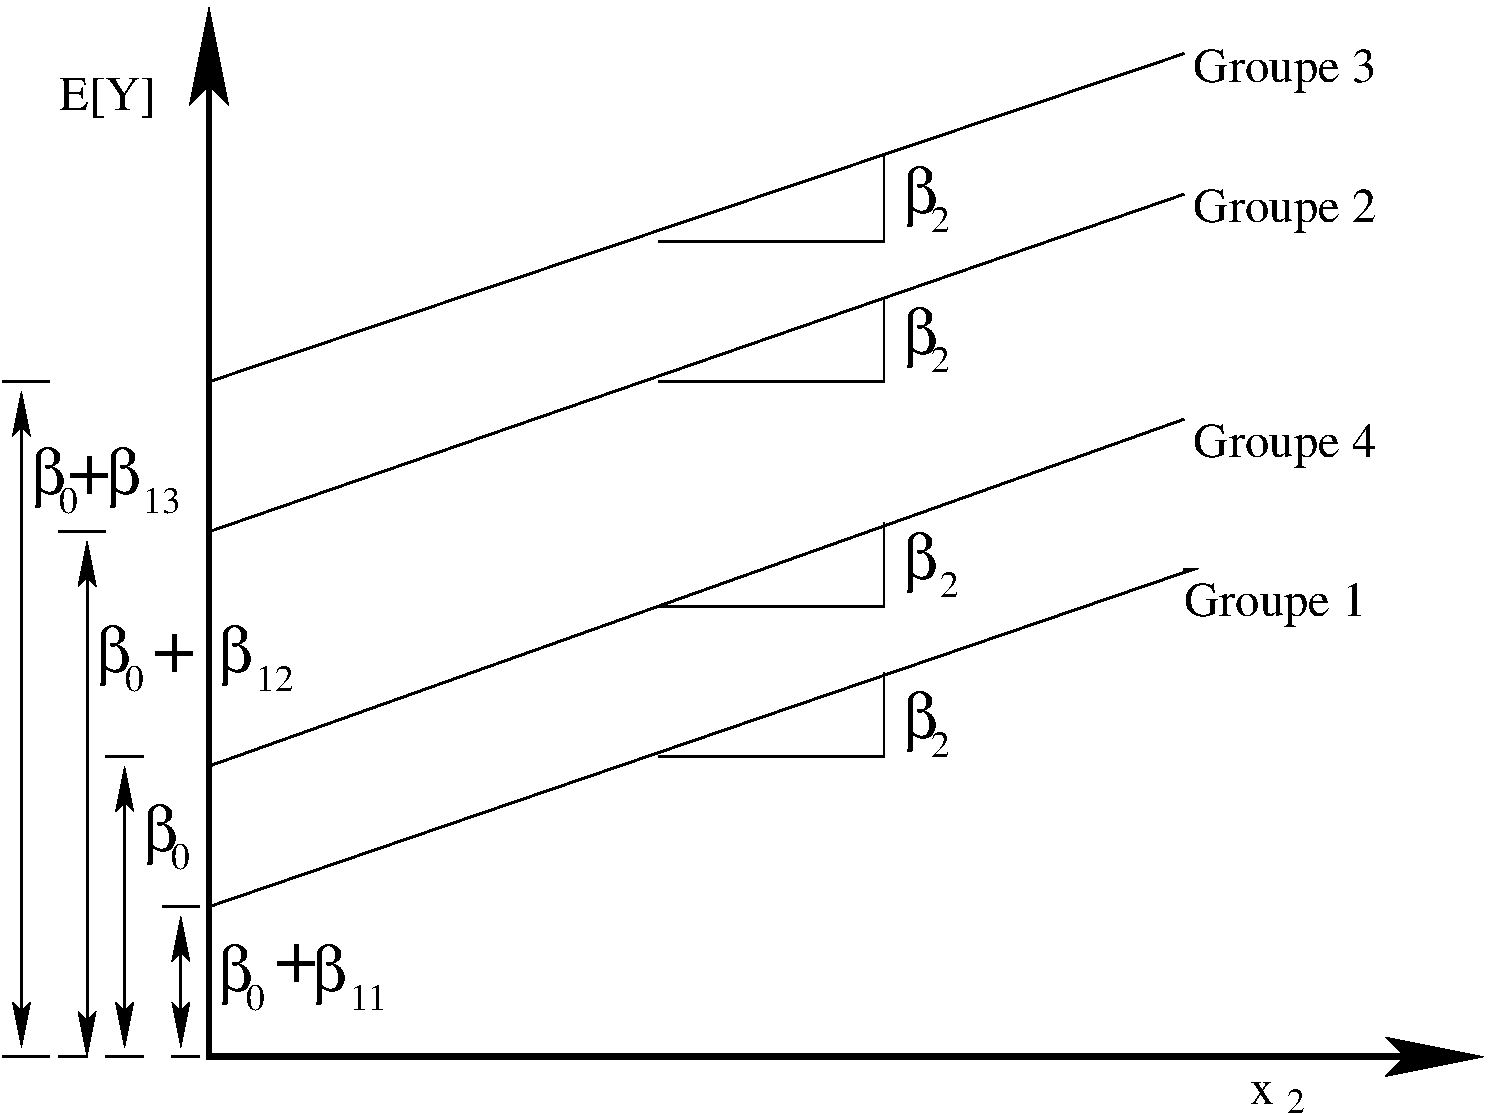
\includegraphics[height=3.5in,angle=0]{Chap7-CategoriquesInteractions/Figures/eyvsx2-eps-converted-to.pdf}}
\caption[Espérance de la variable endogène $Y$ en fonction de
la variable exogène $x_2$ pour chacun des groupes 1 à 4. ]{Espérance de la variable endogène $Y$ en fonction de
la variable exogène $x_2$ pour chacun des groupes 1 à 4. Comme on
peut le voir, les $\beta_0$ et $\beta_{1j}$ déterminent les
ordonnées à l'origine, tandis que $\beta_2$ détermine la
pente des droites de régression.}\label{figex81}
\end{center}
\end{figure}
\end{exemple}


\subsection{Inférence avec des variables catégoriques}

On peut en général faire de l'inférence sur les coefficients des variables indicatrices exactement comme pour les coefficients des variables continues.

\textbf{Tester l'utilité globale d'une variable polytomique}

Il faut toutefois faire attention si on veut tester si une variable polytomique possède un effet significatif
sur la valeur moyenne de la variable endogène. On doit alors tester si
plusieurs coefficients sont simultanément égaux à zéro à
l'aide d'un test $F$ de réduction de modèle. En général, pour tester si une variable polytomique prenant
$C$ valeurs possibles a un effet significatif, il faut tester si
$C-1$ coefficients sont simultanément égaux à zéro.

\begin{exemple}
Supposons que dans le modèle de l'exemple \ref{eg:lot} on souhaite tester si le groupe
d'o\`u provient l'item $i$ a un effet sur la variable dépendante. Il faut alors tester $H_0:\beta_{11}=\beta_{12}=\beta_{13}=0$. Notez que ceci revient à tester si la droite de régression est la m\^eme pour les 4 groupes, c'est-à-dire que sur la figure
\ref{figex81}, les 4 lignes sont superposées.
\end{exemple}

\textbf{Tester une hypothèse plus complexe sur les différents niveaux d'une variable}


Notons aussi que plusieurs hypothèses intéressantes dans un modèle avec variables polytomiques peuvent \^etre vues comme des hypothèses linéaires sur les $\beta$, ce qui nous permet d'utiliser nos résultats de la section \ref{sec:hyplingen}.

\begin{exemple}
Toujours pour le modèle de l'exemple \ref{eg:lot}, supposons qu'on veut tester que la valeur moyenne de $Y_i$ est la m\^eme pour les lots 1 et 3. Ceci revient à tester si $\beta_{11} = \beta_{13}$. On peut donc utiliser un test d'hypothèse linéaire générale avec $$\bo{C} = (0,1,0,-1,0).$$
On pourrait aussi vouloir tester si on peut diviser les lots en deux : les lots 1 et 3 ayant la même moyenne, et les lots 2 et 4 ayant la même moyenne. Ici encore, c'est un test d'hypothèse linéaire générale, mais avec deux contraintes simultanées. La matrice C appropriée est alors:

$$ \bo{C}  =
\begin{bmatrix}
    0 & 1 & 0 & -1 & 0 \\
    0 & 0 & 1 & 0 & 0
\end{bmatrix}.
$$
\end{exemple}




\section{Interactions}

Une interaction entre deux variables exogènes $x_{1i}$ et $x_{2i}$ est un terme de la forme $$\beta_{12}x_{1i}x_{2i}.$$ On inclut une interaction dans un modèle lorsque l'effet d'une des variables sur la moyenne de $Y$ dépend de la valeur d'une autre variable. En effet, supposons le modèle
\vspace{-0.05in}
\begin{equation*}
Y_i=\beta_0+\beta_1x_{1i}+\beta_2x_{2i}+\beta_{12}x_{1i}x_{2i}+
\varepsilon_i.
\end{equation*}
On a alors
\vspace{-0.05in}
\begin{eqnarray}
\esp[Y_i|x_{1i}+1]&=&\beta_0+\beta_1(x_{1i}+1)+\beta_2x_{2i}+\beta_{12}(x_{1i}+1)x_{2i}\label{eq:interaction1}\\
\esp[Y_i|x_{1i}]&=&\beta_0+\beta_1x_{1i}+\beta_2x_{2i}+\beta_{12}x_{1i}x_{2i}.\label{eq:interaction2}
\end{eqnarray}
L'effet d'une augmentation d'une unité de $x_{1i}$ sur $\esp[Y_i]$ est
$\beta_1+\beta_{12}x_{2i}$, c'est-à-dire que l'effet d'une augmentation
de $x_{1i}$ d'une unité sur $\esp[Y_i]$ \textbf{dépend de la valeur
de $x_{2i}$}.

%Alors que l'inclusion d'une variable catégorique dans le modèle modifie l'ordonnée à l'origine, l'inclusion d'une interaction modifie plutôt la pente de la droite ou de l'hyperplan.

\begin{exemple}\label{ex83}
Soit $x_{1i}$ une variable polytomique pouvant prendre les valeurs
$\{1,2,3\}$ et soient $x_{11i}$ l'indicatrice que $x_{1i}=1$ et
$x_{12i}$ l'indicatrice que $x_{1i}=2$. Le modèle
$$Y_i=\beta_0+\beta_{11}x_{11i}+\beta_{12}x_{12i}+\beta_2x_{2i}
+\beta_{112}x_{11i}x_{2i}+\beta_{122}x_{12i}x_{2i}+\varepsilon_i.$$
est illustré à la figure \ref{figex83}.
%Les $\beta_0$ et $\beta_{1ji}$ déterminent les ordonnées à l'origine, tandis que $\beta_2$ et $\beta_{1j2}$ déterminent les pentes des droites de régression.
\begin{figure}[H]
\begin{center}
\centerline{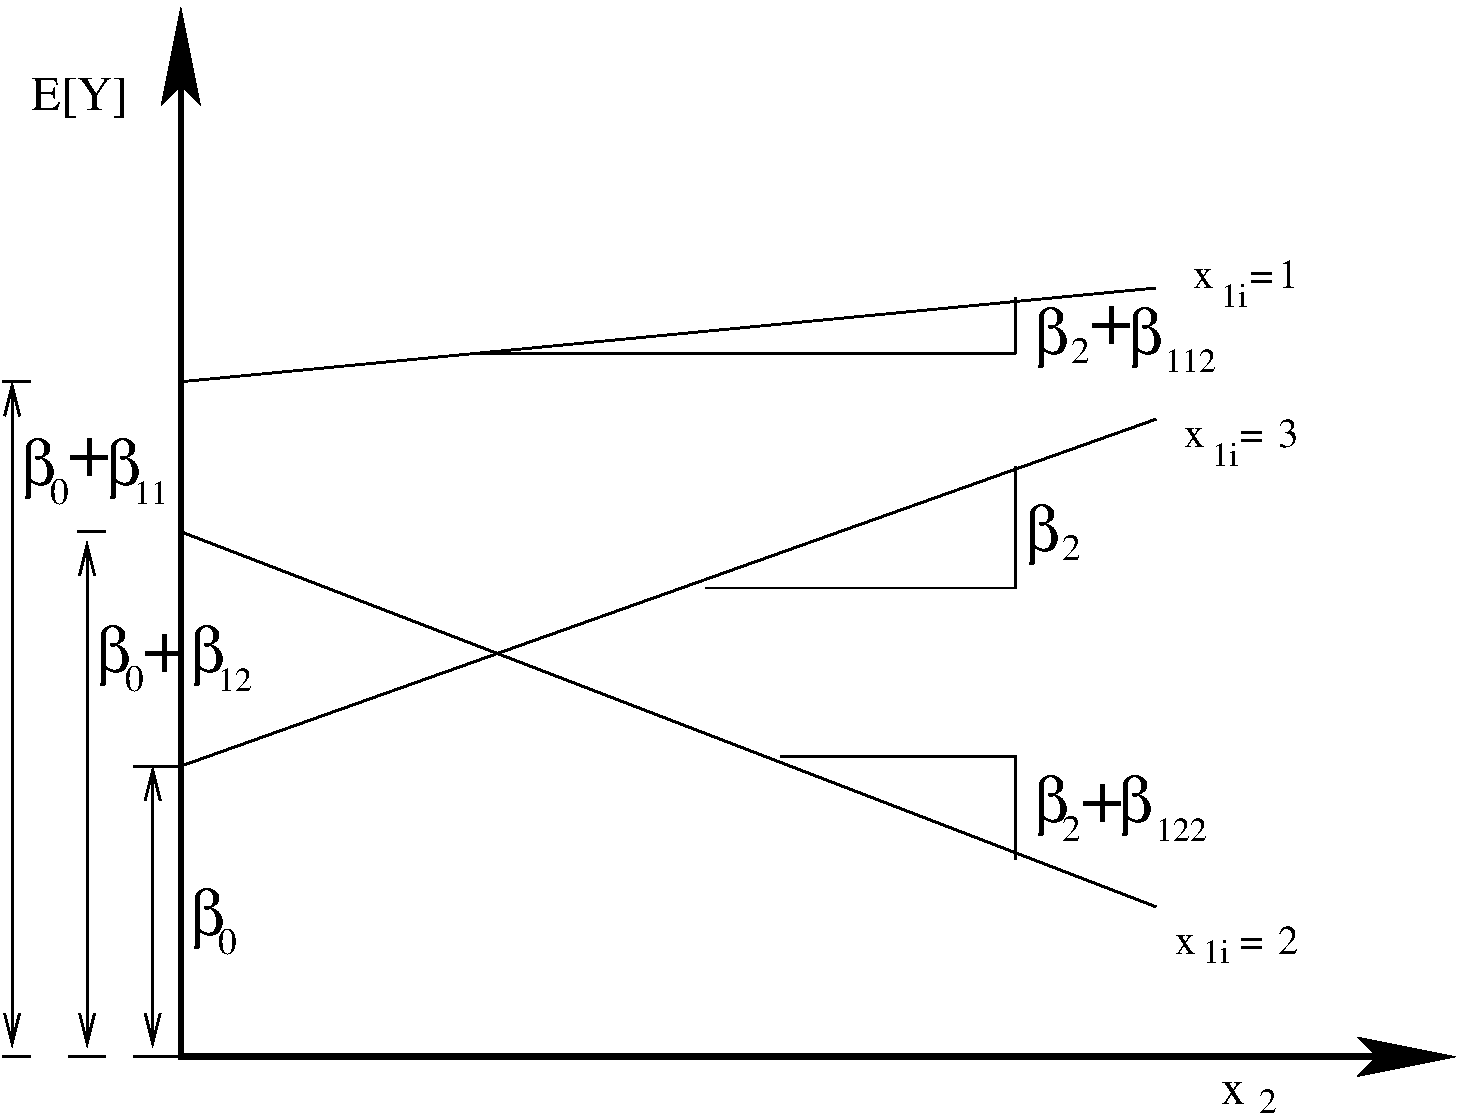
\includegraphics[scale = 0.35]{Chap7-CategoriquesInteractions/Figures/eyvsx2b-eps-converted-to.pdf}}
\caption{Espérance de la variable endogène $Y$ en fonction de
la variable exogène $x_2$ pour chacune des valeurs de $x_{1i}$.
}\label{figex83}
\end{center}\end{figure}
\end{exemple}



L'exemple \ref{ex83} illustre une interaction entre une variable catégorique et une variable continue, ce qui s'illustre aisément. On peut également inclure une interaction entre deux variables catégoriques, ce qui crée en quelque sorte une nouvelle variable catégorique avec plus de catégories. Ou entre deux variables continues, ce qui implique une pente de régression pour une première variable qui diffère pour chaque valeur d'une autre variable.

De plus, les termes d'interaction ne sont pas limités à seulement deux variables. En effet, si nous mesurons 4 variables $x_1,\ldots,x_4$
il se pourrait que le modèle approprié soit
\begin{eqnarray*}
Y_i&=&\beta_0+\beta_1x_{1i}+\beta_2x_{2i}+\beta_3x_{3i}+\beta_4x_{4i}+
\beta_{12}x_{1i}x_{2i}+\beta_{13}x_{1i}x_{3i}\\
&\ &\ \ \ +\beta_{14}x_{1i}x_{4i}+\beta_{23}x_{2i}x_{3i}+
\beta_{24}x_{2i}x_{4i}+\beta_{34}x_{3i}x_{4i}\\
&\ &\ \ \ +\beta_{123}
x_{1i}x_{2i}x_{3i}+\cdots+\beta_{1234}x_{1i}x_{2i}x_{3i}x_{4i}
+\varepsilon_i.\end{eqnarray*} Mais à moins de posséder vraiment beaucoup
de données, les interactions impliquant plus de deux variables
sont rarement utilisées. Elles sont en outre plus complexes à interpréter.


\subsubsection*{Test de linéarité}

Pour tester si un modèle est adéquat, on peut y ajouter des
termes d'interaction et tester si ces termes sont significatifs.
\begin{exemple}
Soit le modèle
$$Y_i=\beta_0+\beta_1x_{1i}+\beta_2x_{2i}+\varepsilon_i.$$ Nous pouvons tester si
$H_0:\ \beta_{12}=0$ contre $H_1:\ \beta_{12}\neq0$ à partir du
modèle
$$Y_i=\beta_0+\beta_1x_{1i}+\beta_2x_{2i}+\beta_{12}x_{1i}x_{2i}+\varepsilon_i.$$
Si nous ne rejetons pas $H_0$, les données ne fournissent pas de preuve suffisante en faveur de cette interaction; cela ne démontre pas que le modèle est adéquat. Si nous rejetons $H_0$, alors le
modèle sans interaction n'est pas adéquat.\\
\end{exemple}

\begin{remarque}
Un cas particulier d'interaction est si on inclut une interaction entre une variable $x_j$ et elle-même, ce qui crée un terme de la forme $x_j^2$ dans l'équation de régression. Ce peut être utile si la relation entre les variables est quadratique plutôt que linéaire. On y reviendra à la section \ref{sec:regpoly}.
\end{remarque} 